\documentclass[twoside]{book}

% Packages required by doxygen
\usepackage{fixltx2e}
\usepackage{calc}
\usepackage{doxygen}
\usepackage[export]{adjustbox} % also loads graphicx
\usepackage{graphicx}
\usepackage[utf8]{inputenc}
\usepackage{makeidx}
\usepackage{multicol}
\usepackage{multirow}
\PassOptionsToPackage{warn}{textcomp}
\usepackage{textcomp}
\usepackage[nointegrals]{wasysym}
\usepackage[table]{xcolor}

% Font selection
\usepackage[T1]{fontenc}
\usepackage[scaled=.90]{helvet}
\usepackage{courier}
\usepackage{amssymb}
\usepackage{sectsty}
\renewcommand{\familydefault}{\sfdefault}
\allsectionsfont{%
  \fontseries{bc}\selectfont%
  \color{darkgray}%
}
\renewcommand{\DoxyLabelFont}{%
  \fontseries{bc}\selectfont%
  \color{darkgray}%
}
\newcommand{\+}{\discretionary{\mbox{\scriptsize$\hookleftarrow$}}{}{}}

% Page & text layout
\usepackage{geometry}
\geometry{%
  a4paper,%
  top=2.5cm,%
  bottom=2.5cm,%
  left=2.5cm,%
  right=2.5cm%
}
\tolerance=750
\hfuzz=15pt
\hbadness=750
\setlength{\emergencystretch}{15pt}
\setlength{\parindent}{0cm}
\setlength{\parskip}{3ex plus 2ex minus 2ex}
\makeatletter
\renewcommand{\paragraph}{%
  \@startsection{paragraph}{4}{0ex}{-1.0ex}{1.0ex}{%
    \normalfont\normalsize\bfseries\SS@parafont%
  }%
}
\renewcommand{\subparagraph}{%
  \@startsection{subparagraph}{5}{0ex}{-1.0ex}{1.0ex}{%
    \normalfont\normalsize\bfseries\SS@subparafont%
  }%
}
\makeatother

% Headers & footers
\usepackage{fancyhdr}
\pagestyle{fancyplain}
\fancyhead[LE]{\fancyplain{}{\bfseries\thepage}}
\fancyhead[CE]{\fancyplain{}{}}
\fancyhead[RE]{\fancyplain{}{\bfseries\leftmark}}
\fancyhead[LO]{\fancyplain{}{\bfseries\rightmark}}
\fancyhead[CO]{\fancyplain{}{}}
\fancyhead[RO]{\fancyplain{}{\bfseries\thepage}}
\fancyfoot[LE]{\fancyplain{}{}}
\fancyfoot[CE]{\fancyplain{}{}}
\fancyfoot[RE]{\fancyplain{}{\bfseries\scriptsize Generated by Doxygen }}
\fancyfoot[LO]{\fancyplain{}{\bfseries\scriptsize Generated by Doxygen }}
\fancyfoot[CO]{\fancyplain{}{}}
\fancyfoot[RO]{\fancyplain{}{}}
\renewcommand{\footrulewidth}{0.4pt}
\renewcommand{\chaptermark}[1]{%
  \markboth{#1}{}%
}
\renewcommand{\sectionmark}[1]{%
  \markright{\thesection\ #1}%
}

% Indices & bibliography
\usepackage{natbib}
\usepackage[titles]{tocloft}
\setcounter{tocdepth}{3}
\setcounter{secnumdepth}{5}
\makeindex

% Hyperlinks (required, but should be loaded last)
\usepackage{ifpdf}
\ifpdf
  \usepackage[pdftex,pagebackref=true]{hyperref}
\else
  \usepackage[ps2pdf,pagebackref=true]{hyperref}
\fi
\hypersetup{%
  colorlinks=true,%
  linkcolor=blue,%
  citecolor=blue,%
  unicode%
}

% Custom commands
\newcommand{\clearemptydoublepage}{%
  \newpage{\pagestyle{empty}\cleardoublepage}%
}

\usepackage{caption}
\captionsetup{labelsep=space,justification=centering,font={bf},singlelinecheck=off,skip=4pt,position=top}

%===== C O N T E N T S =====

\begin{document}

% Titlepage & ToC
\hypersetup{pageanchor=false,
             bookmarksnumbered=true,
             pdfencoding=unicode
            }
\pagenumbering{alph}
\begin{titlepage}
\vspace*{7cm}
\begin{center}%
{\Large Proyecto0 Manipulación de imagenes digitales \\[1ex]\large 1.\+0 }\\
\vspace*{1cm}
{\large Generated by Doxygen 1.8.13}\\
\end{center}
\end{titlepage}
\clearemptydoublepage
\pagenumbering{roman}
\tableofcontents
\clearemptydoublepage
\pagenumbering{arabic}
\hypersetup{pageanchor=true}

%--- Begin generated contents ---
\chapter{Class Index}
\section{Class List}
Here are the classes, structs, unions and interfaces with brief descriptions\+:\begin{DoxyCompactList}
\item\contentsline{section}{\hyperlink{class_binary_search_tree}{Binary\+Search\+Tree$<$ Data, Type\+Nodo $>$} }{\pageref{class_binary_search_tree}}{}
\item\contentsline{section}{\hyperlink{class_circulo}{Circulo} \\*Clase que se encarga e modelar un circulo }{\pageref{class_circulo}}{}
\item\contentsline{section}{\hyperlink{class_class_node}{Class\+Node$<$ Dato $>$} }{\pageref{class_class_node}}{}
\item\contentsline{section}{\hyperlink{class_dato_no_primitivo}{Dato\+No\+Primitivo$<$ Tipo\+Dato $>$} }{\pageref{class_dato_no_primitivo}}{}
\item\contentsline{section}{\hyperlink{class_equilatero}{Equilatero} \\*Calse equilatero }{\pageref{class_equilatero}}{}
\item\contentsline{section}{\hyperlink{class_escaleno}{Escaleno} \\*Calse \hyperlink{class_escaleno}{Escaleno} }{\pageref{class_escaleno}}{}
\item\contentsline{section}{\hyperlink{class_figura}{Figura} \\*Clase que se encarga de crear una figura en 2D }{\pageref{class_figura}}{}
\item\contentsline{section}{\hyperlink{class_impresora}{Impresora$<$ T $>$} \\*Clase que imprmime objetos }{\pageref{class_impresora}}{}
\item\contentsline{section}{\hyperlink{class_isosceles}{Isosceles} \\*Calse \hyperlink{class_isosceles}{Isosceles} }{\pageref{class_isosceles}}{}
\item\contentsline{section}{\hyperlink{class_principal}{Principal} }{\pageref{class_principal}}{}
\item\contentsline{section}{\hyperlink{classrectangulo}{rectangulo} \\*Clase rectangulo }{\pageref{classrectangulo}}{}
\item\contentsline{section}{\hyperlink{classtriangulo}{triangulo} \\*Calse tringulo }{\pageref{classtriangulo}}{}
\item\contentsline{section}{\hyperlink{class_vertice}{Vertice} \\*Clase que modela un punto en el espacio }{\pageref{class_vertice}}{}
\end{DoxyCompactList}

\chapter{File Index}
\section{File List}
Here is a list of all documented files with brief descriptions\+:\begin{DoxyCompactList}
\item\contentsline{section}{\hyperlink{main_8cpp}{main.\+cpp} \\*Archivo pricipal, Proyecto final, Programacion bajo plataformas abiertas }{\pageref{main_8cpp}}{}
\item\contentsline{section}{include/{\bfseries Includes.\+h} }{\pageref{_includes_8h}}{}
\item\contentsline{section}{include/{\bfseries tools.\+h} }{\pageref{tools_8h}}{}
\item\contentsline{section}{sample/\hyperlink{_comprobar_gesto_8cpp}{Comprobar\+Gesto.\+cpp} \\*Archivo que permite comprobar cada frame del leap con el guardo en la base de datos, se toma como base el ejemplo dado en el sdk y se le realizan modificaciones }{\pageref{_comprobar_gesto_8cpp}}{}
\item\contentsline{section}{sample/include/{\bfseries Leap.\+h} }{\pageref{_leap_8h}}{}
\item\contentsline{section}{sample/include/{\bfseries Leap\+Math.\+h} }{\pageref{_leap_math_8h}}{}
\item\contentsline{section}{sourcecode/\hyperlink{tools_8cpp}{tools.\+cpp} \\*Archivo que contiene funciones utiles para el main }{\pageref{tools_8cpp}}{}
\end{DoxyCompactList}

\chapter{Class Documentation}
\hypertarget{class_filtros}{}\section{Filtros Class Reference}
\label{class_filtros}\index{Filtros@{Filtros}}


Clase que controla todos los filtros.  




{\ttfamily \#include $<$Filtros.\+hpp$>$}

\subsection*{Public Member Functions}
\begin{DoxyCompactItemize}
\item 
\hyperlink{class_filtros_ada24dd279d9c0e4c95738162866bd261}{Filtros} (string imagen)
\begin{DoxyCompactList}\small\item\em constructor \end{DoxyCompactList}\item 
\hyperlink{class_filtros_a5d4383dece49dcc80b3ce18da579a338}{Filtros} ()
\begin{DoxyCompactList}\small\item\em constructor por defecto \end{DoxyCompactList}\item 
\hyperlink{class_filtros_ae0486e405aaac60c6f19eaef6b3b01df}{$\sim$\+Filtros} ()
\begin{DoxyCompactList}\small\item\em destructor \end{DoxyCompactList}\item 
void \hyperlink{class_filtros_a176534ec297bdde49cb959602eea0d29}{Filtro\+Gaussiano} ()
\begin{DoxyCompactList}\small\item\em Genera un filtro gausiano. \end{DoxyCompactList}\item 
void \hyperlink{class_filtros_a63c1da79fb2190ae07b354ee4ee67819}{Filtro\+Gaussiano\+Un\+Canal} ()
\begin{DoxyCompactList}\small\item\em Genera un filtro gausiano para imagenes de un canal. \end{DoxyCompactList}\item 
void \hyperlink{class_filtros_a81e2f015d497d80032af22f471b360eb}{Filtro\+Desviacion\+Estandar} ()
\begin{DoxyCompactList}\small\item\em Funcion que realiza el filtro de desviavion estandar. \end{DoxyCompactList}\item 
void \hyperlink{class_filtros_a9bed709d7363047dc9ec1449c4dd00b4}{Deteccion\+Bordes} ()
\begin{DoxyCompactList}\small\item\em calcula los bordes de una imagen \end{DoxyCompactList}\item 
void \hyperlink{class_filtros_a5826f19a9932e321c29fd1efa9c70e4d}{Difuminado\+Movimiento} ()
\begin{DoxyCompactList}\small\item\em Filtro de movimiento. \end{DoxyCompactList}\item 
void \hyperlink{class_filtros_a2ad4f5b18c537599bc171b9799683b1a}{Ruido\+Sal\+Pimienta} (float)
\begin{DoxyCompactList}\small\item\em Creal el filtro sal y pimienta. \end{DoxyCompactList}\item 
void \hyperlink{class_filtros_a8f604a50556e0e06e707cee8055522d1}{Erosion} ()
\begin{DoxyCompactList}\small\item\em Crea el filtro de erosion. \end{DoxyCompactList}\item 
void \hyperlink{class_filtros_a6b296610ee0b6f782d9be9f8c4ad25c2}{Dilatacion} ()
\begin{DoxyCompactList}\small\item\em Crea el filtro de dilatacion. \end{DoxyCompactList}\item 
void \hyperlink{class_filtros_a729e3fca9fd6ab3d39c3ae579ab26737}{Inversion\+Color} ()
\begin{DoxyCompactList}\small\item\em Genera un filtro negativo. \end{DoxyCompactList}\item 
void \hyperlink{class_filtros_a19ec703cb72322ef5cb7a38aa7de5c7b}{Transformacion\+Escala\+Grises} ()
\begin{DoxyCompactList}\small\item\em Genera un filtro en escala de grises. \end{DoxyCompactList}\item 
void \hyperlink{class_filtros_a85e035d3ce1a721331aba30535487a57}{Binario} ()
\begin{DoxyCompactList}\small\item\em Crea el filtro de imagen binaria. \end{DoxyCompactList}\item 
void \hyperlink{class_filtros_a69d9e93f385d769a769b25033472bd67}{Escribir\+Imagen} (string, string, string)
\begin{DoxyCompactList}\small\item\em Funcion que escribe una imagen. \end{DoxyCompactList}\end{DoxyCompactItemize}
\subsection*{Public Attributes}
\begin{DoxyCompactItemize}
\item 
Mat \hyperlink{class_filtros_a7bb45c07cea0bed3d4a4b8a7cca38fe9}{matriz\+Imagen}
\end{DoxyCompactItemize}


\subsection{Detailed Description}
Clase que controla todos los filtros. 

\subsection{Constructor \& Destructor Documentation}
\mbox{\Hypertarget{class_filtros_ada24dd279d9c0e4c95738162866bd261}\label{class_filtros_ada24dd279d9c0e4c95738162866bd261}} 
\index{Filtros@{Filtros}!Filtros@{Filtros}}
\index{Filtros@{Filtros}!Filtros@{Filtros}}
\subsubsection{\texorpdfstring{Filtros()}{Filtros()}\hspace{0.1cm}{\footnotesize\ttfamily [1/2]}}
{\footnotesize\ttfamily Filtros\+::\+Filtros (\begin{DoxyParamCaption}\item[{string}]{imagen }\end{DoxyParamCaption})\hspace{0.3cm}{\ttfamily [inline]}}



constructor 

\mbox{\Hypertarget{class_filtros_a5d4383dece49dcc80b3ce18da579a338}\label{class_filtros_a5d4383dece49dcc80b3ce18da579a338}} 
\index{Filtros@{Filtros}!Filtros@{Filtros}}
\index{Filtros@{Filtros}!Filtros@{Filtros}}
\subsubsection{\texorpdfstring{Filtros()}{Filtros()}\hspace{0.1cm}{\footnotesize\ttfamily [2/2]}}
{\footnotesize\ttfamily Filtros\+::\+Filtros (\begin{DoxyParamCaption}{ }\end{DoxyParamCaption})\hspace{0.3cm}{\ttfamily [inline]}}



constructor por defecto 

\mbox{\Hypertarget{class_filtros_ae0486e405aaac60c6f19eaef6b3b01df}\label{class_filtros_ae0486e405aaac60c6f19eaef6b3b01df}} 
\index{Filtros@{Filtros}!````~Filtros@{$\sim$\+Filtros}}
\index{````~Filtros@{$\sim$\+Filtros}!Filtros@{Filtros}}
\subsubsection{\texorpdfstring{$\sim$\+Filtros()}{~Filtros()}}
{\footnotesize\ttfamily Filtros\+::$\sim$\+Filtros (\begin{DoxyParamCaption}{ }\end{DoxyParamCaption})\hspace{0.3cm}{\ttfamily [inline]}}



destructor 



\subsection{Member Function Documentation}
\mbox{\Hypertarget{class_filtros_a85e035d3ce1a721331aba30535487a57}\label{class_filtros_a85e035d3ce1a721331aba30535487a57}} 
\index{Filtros@{Filtros}!Binario@{Binario}}
\index{Binario@{Binario}!Filtros@{Filtros}}
\subsubsection{\texorpdfstring{Binario()}{Binario()}}
{\footnotesize\ttfamily void Filtros\+::\+Binario (\begin{DoxyParamCaption}{ }\end{DoxyParamCaption})}



Crea el filtro de imagen binaria. 

\mbox{\Hypertarget{class_filtros_a9bed709d7363047dc9ec1449c4dd00b4}\label{class_filtros_a9bed709d7363047dc9ec1449c4dd00b4}} 
\index{Filtros@{Filtros}!Deteccion\+Bordes@{Deteccion\+Bordes}}
\index{Deteccion\+Bordes@{Deteccion\+Bordes}!Filtros@{Filtros}}
\subsubsection{\texorpdfstring{Deteccion\+Bordes()}{DeteccionBordes()}}
{\footnotesize\ttfamily void Filtros\+::\+Deteccion\+Bordes (\begin{DoxyParamCaption}{ }\end{DoxyParamCaption})}



calcula los bordes de una imagen 

\mbox{\Hypertarget{class_filtros_a5826f19a9932e321c29fd1efa9c70e4d}\label{class_filtros_a5826f19a9932e321c29fd1efa9c70e4d}} 
\index{Filtros@{Filtros}!Difuminado\+Movimiento@{Difuminado\+Movimiento}}
\index{Difuminado\+Movimiento@{Difuminado\+Movimiento}!Filtros@{Filtros}}
\subsubsection{\texorpdfstring{Difuminado\+Movimiento()}{DifuminadoMovimiento()}}
{\footnotesize\ttfamily void Filtros\+::\+Difuminado\+Movimiento (\begin{DoxyParamCaption}{ }\end{DoxyParamCaption})}



Filtro de movimiento. 

\mbox{\Hypertarget{class_filtros_a6b296610ee0b6f782d9be9f8c4ad25c2}\label{class_filtros_a6b296610ee0b6f782d9be9f8c4ad25c2}} 
\index{Filtros@{Filtros}!Dilatacion@{Dilatacion}}
\index{Dilatacion@{Dilatacion}!Filtros@{Filtros}}
\subsubsection{\texorpdfstring{Dilatacion()}{Dilatacion()}}
{\footnotesize\ttfamily void Filtros\+::\+Dilatacion (\begin{DoxyParamCaption}{ }\end{DoxyParamCaption})}



Crea el filtro de dilatacion. 

brief Crea el filtro de dilatacion

void \hyperlink{class_filtros_a6b296610ee0b6f782d9be9f8c4ad25c2}{Filtros\+::\+Dilatacion()}\{ Mat imagen = matriz\+Imagen; Mat nueva(imagen.\+rows, imagen.\+cols, C\+V\+\_\+8\+U\+C3); Vec3b pixel; Vec3b blanco = \{255,255,255\}; Vec3b negro = \{0,0,0\}; for (int i=0; i$<$imagen.\+rows; i++)\{ for (int j=0; j$<$imagen.\+cols; j++)\{ pixel=imagen.\+at$<$\+Vec3b$>$(i, j); double gris = pixel\mbox{[}0\mbox{]}$\ast$0.3 + pixel\mbox{[}1\mbox{]}$\ast$0.59+pixel\mbox{[}2\mbox{]}$\ast$0.11; if (gris $>$127)\{ nueva.\+at$<$\+Vec3b$>$(i, j)=blanco; \}else\{ nueva.\+at$<$\+Vec3b$>$(i, j)=negro; \} \} \} \mbox{\Hypertarget{class_filtros_a8f604a50556e0e06e707cee8055522d1}\label{class_filtros_a8f604a50556e0e06e707cee8055522d1}} 
\index{Filtros@{Filtros}!Erosion@{Erosion}}
\index{Erosion@{Erosion}!Filtros@{Filtros}}
\subsubsection{\texorpdfstring{Erosion()}{Erosion()}}
{\footnotesize\ttfamily void Filtros\+::\+Erosion (\begin{DoxyParamCaption}{ }\end{DoxyParamCaption})}



Crea el filtro de erosion. 

\mbox{\Hypertarget{class_filtros_a69d9e93f385d769a769b25033472bd67}\label{class_filtros_a69d9e93f385d769a769b25033472bd67}} 
\index{Filtros@{Filtros}!Escribir\+Imagen@{Escribir\+Imagen}}
\index{Escribir\+Imagen@{Escribir\+Imagen}!Filtros@{Filtros}}
\subsubsection{\texorpdfstring{Escribir\+Imagen()}{EscribirImagen()}}
{\footnotesize\ttfamily void Filtros\+::\+Escribir\+Imagen (\begin{DoxyParamCaption}\item[{string}]{imagen,  }\item[{string}]{filtro,  }\item[{string}]{formato }\end{DoxyParamCaption})}



Funcion que escribe una imagen. 


\begin{DoxyParams}{Parameters}
{\em imagen} & es la imagen original \\
\hline
{\em filtro} & es el filtro aplocado \\
\hline
{\em formato} & es el formato de salida \\
\hline
\end{DoxyParams}
\mbox{\Hypertarget{class_filtros_a81e2f015d497d80032af22f471b360eb}\label{class_filtros_a81e2f015d497d80032af22f471b360eb}} 
\index{Filtros@{Filtros}!Filtro\+Desviacion\+Estandar@{Filtro\+Desviacion\+Estandar}}
\index{Filtro\+Desviacion\+Estandar@{Filtro\+Desviacion\+Estandar}!Filtros@{Filtros}}
\subsubsection{\texorpdfstring{Filtro\+Desviacion\+Estandar()}{FiltroDesviacionEstandar()}}
{\footnotesize\ttfamily void Filtros\+::\+Filtro\+Desviacion\+Estandar (\begin{DoxyParamCaption}{ }\end{DoxyParamCaption})}



Funcion que realiza el filtro de desviavion estandar. 

\mbox{\Hypertarget{class_filtros_a176534ec297bdde49cb959602eea0d29}\label{class_filtros_a176534ec297bdde49cb959602eea0d29}} 
\index{Filtros@{Filtros}!Filtro\+Gaussiano@{Filtro\+Gaussiano}}
\index{Filtro\+Gaussiano@{Filtro\+Gaussiano}!Filtros@{Filtros}}
\subsubsection{\texorpdfstring{Filtro\+Gaussiano()}{FiltroGaussiano()}}
{\footnotesize\ttfamily void Filtros\+::\+Filtro\+Gaussiano (\begin{DoxyParamCaption}{ }\end{DoxyParamCaption})}



Genera un filtro gausiano. 

\mbox{\Hypertarget{class_filtros_a63c1da79fb2190ae07b354ee4ee67819}\label{class_filtros_a63c1da79fb2190ae07b354ee4ee67819}} 
\index{Filtros@{Filtros}!Filtro\+Gaussiano\+Un\+Canal@{Filtro\+Gaussiano\+Un\+Canal}}
\index{Filtro\+Gaussiano\+Un\+Canal@{Filtro\+Gaussiano\+Un\+Canal}!Filtros@{Filtros}}
\subsubsection{\texorpdfstring{Filtro\+Gaussiano\+Un\+Canal()}{FiltroGaussianoUnCanal()}}
{\footnotesize\ttfamily void Filtros\+::\+Filtro\+Gaussiano\+Un\+Canal (\begin{DoxyParamCaption}{ }\end{DoxyParamCaption})}



Genera un filtro gausiano para imagenes de un canal. 

\mbox{\Hypertarget{class_filtros_a729e3fca9fd6ab3d39c3ae579ab26737}\label{class_filtros_a729e3fca9fd6ab3d39c3ae579ab26737}} 
\index{Filtros@{Filtros}!Inversion\+Color@{Inversion\+Color}}
\index{Inversion\+Color@{Inversion\+Color}!Filtros@{Filtros}}
\subsubsection{\texorpdfstring{Inversion\+Color()}{InversionColor()}}
{\footnotesize\ttfamily void Filtros\+::\+Inversion\+Color (\begin{DoxyParamCaption}{ }\end{DoxyParamCaption})}



Genera un filtro negativo. 

\mbox{\Hypertarget{class_filtros_a2ad4f5b18c537599bc171b9799683b1a}\label{class_filtros_a2ad4f5b18c537599bc171b9799683b1a}} 
\index{Filtros@{Filtros}!Ruido\+Sal\+Pimienta@{Ruido\+Sal\+Pimienta}}
\index{Ruido\+Sal\+Pimienta@{Ruido\+Sal\+Pimienta}!Filtros@{Filtros}}
\subsubsection{\texorpdfstring{Ruido\+Sal\+Pimienta()}{RuidoSalPimienta()}}
{\footnotesize\ttfamily void Filtros\+::\+Ruido\+Sal\+Pimienta (\begin{DoxyParamCaption}\item[{float}]{porciento }\end{DoxyParamCaption})}



Creal el filtro sal y pimienta. 


\begin{DoxyParams}{Parameters}
{\em porciento} & es el porcentaje de aleatoriedad del filtro \\
\hline
\end{DoxyParams}
\mbox{\Hypertarget{class_filtros_a19ec703cb72322ef5cb7a38aa7de5c7b}\label{class_filtros_a19ec703cb72322ef5cb7a38aa7de5c7b}} 
\index{Filtros@{Filtros}!Transformacion\+Escala\+Grises@{Transformacion\+Escala\+Grises}}
\index{Transformacion\+Escala\+Grises@{Transformacion\+Escala\+Grises}!Filtros@{Filtros}}
\subsubsection{\texorpdfstring{Transformacion\+Escala\+Grises()}{TransformacionEscalaGrises()}}
{\footnotesize\ttfamily void Filtros\+::\+Transformacion\+Escala\+Grises (\begin{DoxyParamCaption}{ }\end{DoxyParamCaption})}



Genera un filtro en escala de grises. 



\subsection{Member Data Documentation}
\mbox{\Hypertarget{class_filtros_a7bb45c07cea0bed3d4a4b8a7cca38fe9}\label{class_filtros_a7bb45c07cea0bed3d4a4b8a7cca38fe9}} 
\index{Filtros@{Filtros}!matriz\+Imagen@{matriz\+Imagen}}
\index{matriz\+Imagen@{matriz\+Imagen}!Filtros@{Filtros}}
\subsubsection{\texorpdfstring{matriz\+Imagen}{matrizImagen}}
{\footnotesize\ttfamily Mat Filtros\+::matriz\+Imagen}



The documentation for this class was generated from the following files\+:\begin{DoxyCompactItemize}
\item 
include/\hyperlink{_filtros_8hpp}{Filtros.\+hpp}\item 
sourcecode/\hyperlink{_filtros_8cpp}{Filtros.\+cpp}\end{DoxyCompactItemize}

\chapter{File Documentation}
\hypertarget{_filtros_8hpp}{}\section{include/\+Filtros.hpp File Reference}
\label{_filtros_8hpp}\index{include/\+Filtros.\+hpp@{include/\+Filtros.\+hpp}}
{\ttfamily \#include \char`\"{}./\+Includes.\+hpp\char`\"{}}\newline
Include dependency graph for Filtros.\+hpp\+:
\nopagebreak
\begin{figure}[H]
\begin{center}
\leavevmode
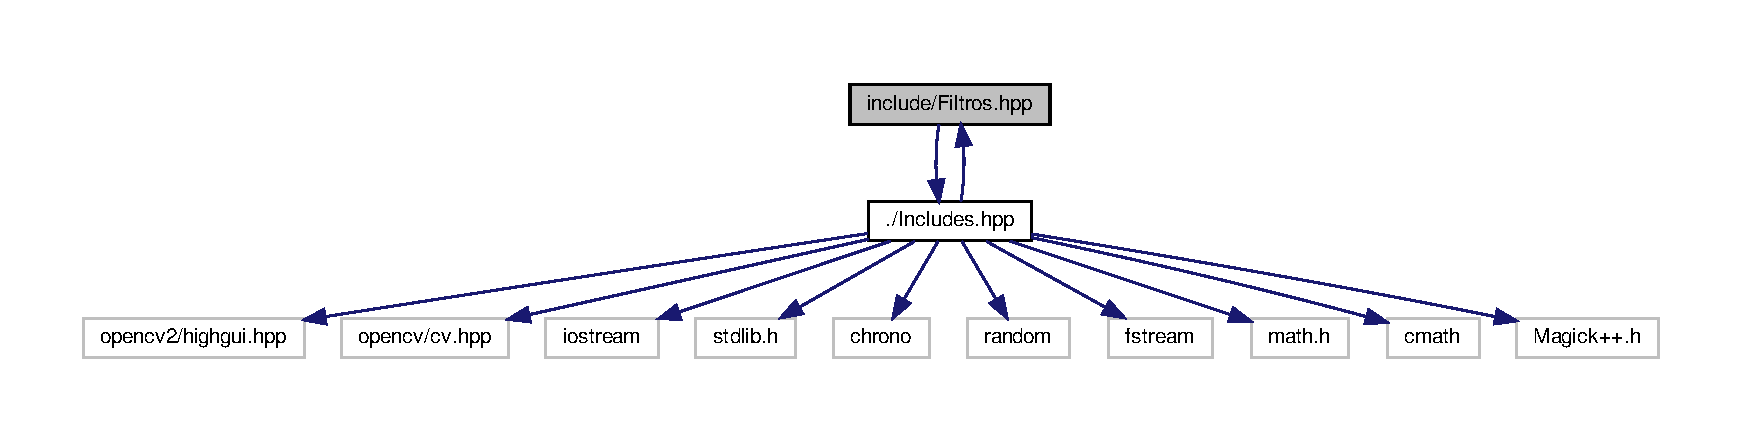
\includegraphics[width=350pt]{_filtros_8hpp__incl}
\end{center}
\end{figure}
This graph shows which files directly or indirectly include this file\+:
\nopagebreak
\begin{figure}[H]
\begin{center}
\leavevmode
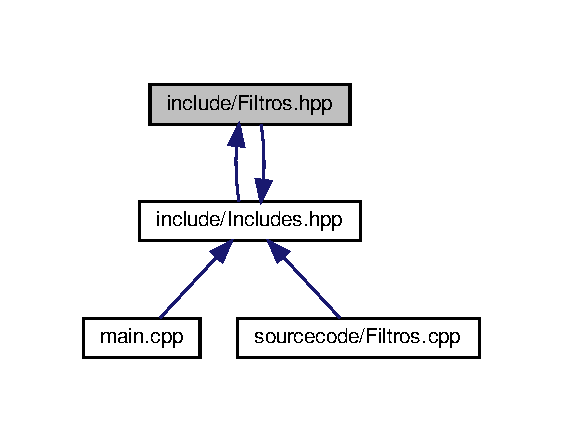
\includegraphics[width=270pt]{_filtros_8hpp__dep__incl}
\end{center}
\end{figure}
\subsection*{Classes}
\begin{DoxyCompactItemize}
\item 
class \hyperlink{class_filtros}{Filtros}
\begin{DoxyCompactList}\small\item\em Clase que controla todos los filtros. \end{DoxyCompactList}\end{DoxyCompactItemize}


\subsection{Detailed Description}
/ 
\hypertarget{_includes_8hpp}{}\section{include/\+Includes.hpp File Reference}
\label{_includes_8hpp}\index{include/\+Includes.\+hpp@{include/\+Includes.\+hpp}}
{\ttfamily \#include $<$opencv2/highgui.\+hpp$>$}\newline
{\ttfamily \#include $<$opencv/cv.\+hpp$>$}\newline
{\ttfamily \#include $<$iostream$>$}\newline
{\ttfamily \#include $<$stdlib.\+h$>$}\newline
{\ttfamily \#include $<$chrono$>$}\newline
{\ttfamily \#include $<$random$>$}\newline
{\ttfamily \#include $<$fstream$>$}\newline
{\ttfamily \#include $<$math.\+h$>$}\newline
{\ttfamily \#include $<$cmath$>$}\newline
{\ttfamily \#include \char`\"{}./\+Filtros.\+hpp\char`\"{}}\newline
{\ttfamily \#include $<$Magick++.\+h$>$}\newline
Include dependency graph for Includes.\+hpp\+:
\nopagebreak
\begin{figure}[H]
\begin{center}
\leavevmode
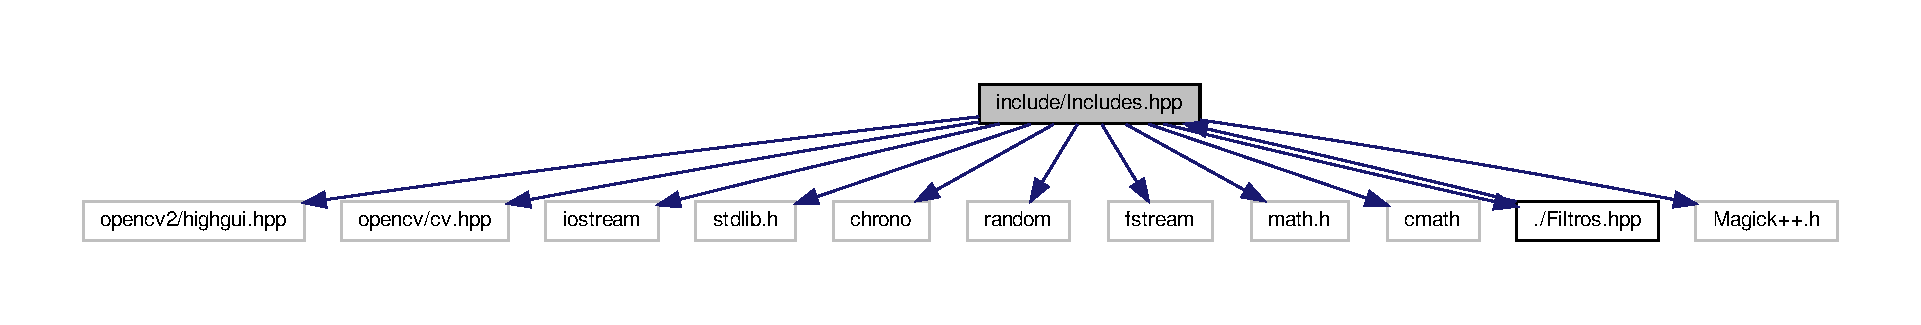
\includegraphics[width=350pt]{_includes_8hpp__incl}
\end{center}
\end{figure}
This graph shows which files directly or indirectly include this file\+:
\nopagebreak
\begin{figure}[H]
\begin{center}
\leavevmode
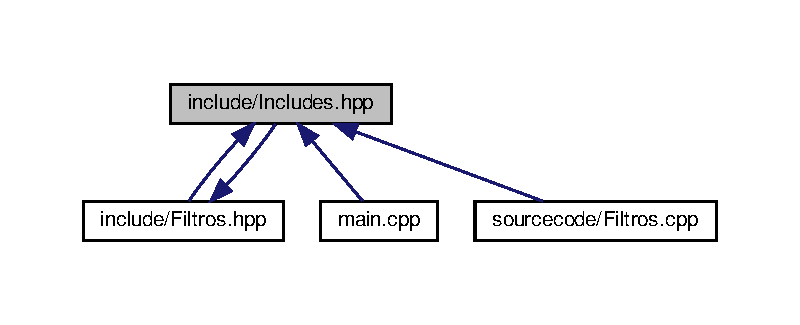
\includegraphics[width=350pt]{_includes_8hpp__dep__incl}
\end{center}
\end{figure}


\subsection{Detailed Description}
/ 
\hypertarget{main_8cpp}{}\section{main.\+cpp File Reference}
\label{main_8cpp}\index{main.\+cpp@{main.\+cpp}}


Archivo pricipal, Proyecto final, Programacion bajo plataformas abiertas.  


{\ttfamily \#include \char`\"{}./include/\+Includes.\+h\char`\"{}}\newline
Include dependency graph for main.\+cpp\+:

\hypertarget{_filtros_8cpp}{}\section{sourcecode/\+Filtros.cpp File Reference}
\label{_filtros_8cpp}\index{sourcecode/\+Filtros.\+cpp@{sourcecode/\+Filtros.\+cpp}}
{\ttfamily \#include \char`\"{}../include/\+Includes.\+hpp\char`\"{}}\newline
Include dependency graph for Filtros.\+cpp\+:
\nopagebreak
\begin{figure}[H]
\begin{center}
\leavevmode
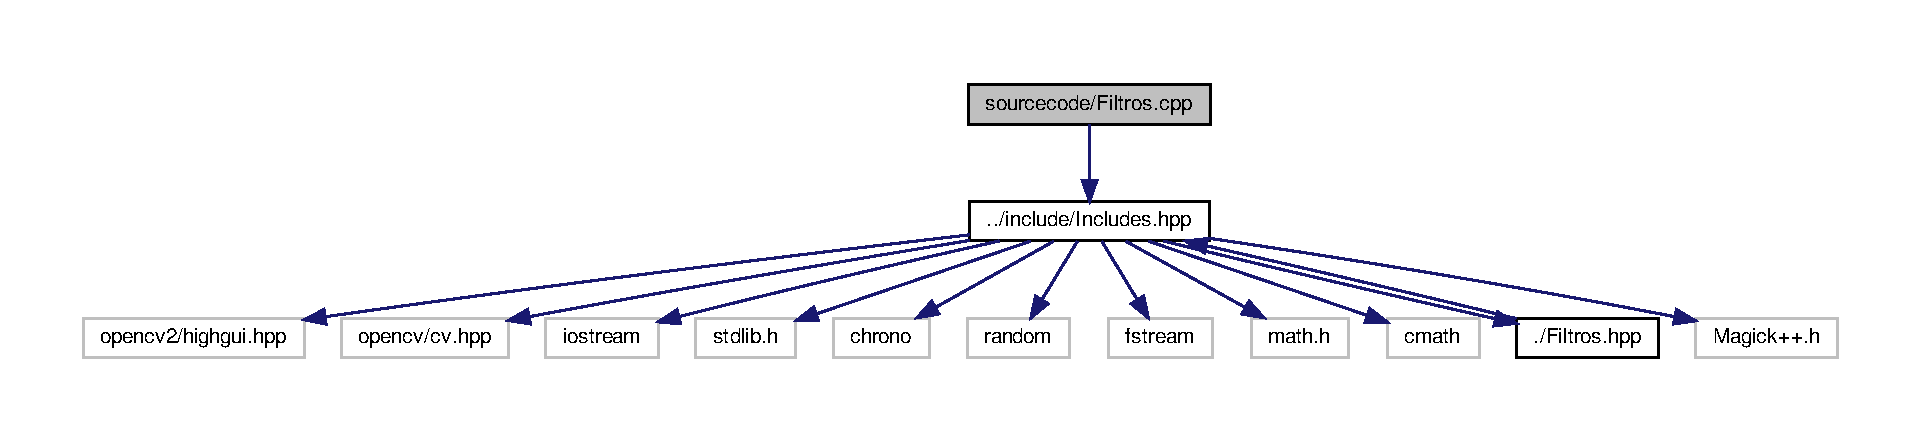
\includegraphics[width=350pt]{_filtros_8cpp__incl}
\end{center}
\end{figure}
\subsection*{Functions}
\begin{DoxyCompactItemize}
\item 
int \hyperlink{_filtros_8cpp_a38914e32c0a41e79795b9f4b97e17cfa}{numero\+Random} (int tope)
\begin{DoxyCompactList}\small\item\em genera un numero aleatorio con distribucion uniforme \end{DoxyCompactList}\end{DoxyCompactItemize}


\subsection{Function Documentation}
\mbox{\Hypertarget{_filtros_8cpp_a38914e32c0a41e79795b9f4b97e17cfa}\label{_filtros_8cpp_a38914e32c0a41e79795b9f4b97e17cfa}} 
\index{Filtros.\+cpp@{Filtros.\+cpp}!numero\+Random@{numero\+Random}}
\index{numero\+Random@{numero\+Random}!Filtros.\+cpp@{Filtros.\+cpp}}
\subsubsection{\texorpdfstring{numero\+Random()}{numeroRandom()}}
{\footnotesize\ttfamily int numero\+Random (\begin{DoxyParamCaption}\item[{int}]{tope }\end{DoxyParamCaption})}



genera un numero aleatorio con distribucion uniforme 


\begin{DoxyParams}{Parameters}
{\em tope} & es el numero mayor que se va a generar \\
\hline
\end{DoxyParams}

%--- End generated contents ---

% Index
\backmatter
\newpage
\phantomsection
\clearemptydoublepage
\addcontentsline{toc}{chapter}{Index}
\printindex

\end{document}
